\usetikzlibrary{arrows.meta,calc}
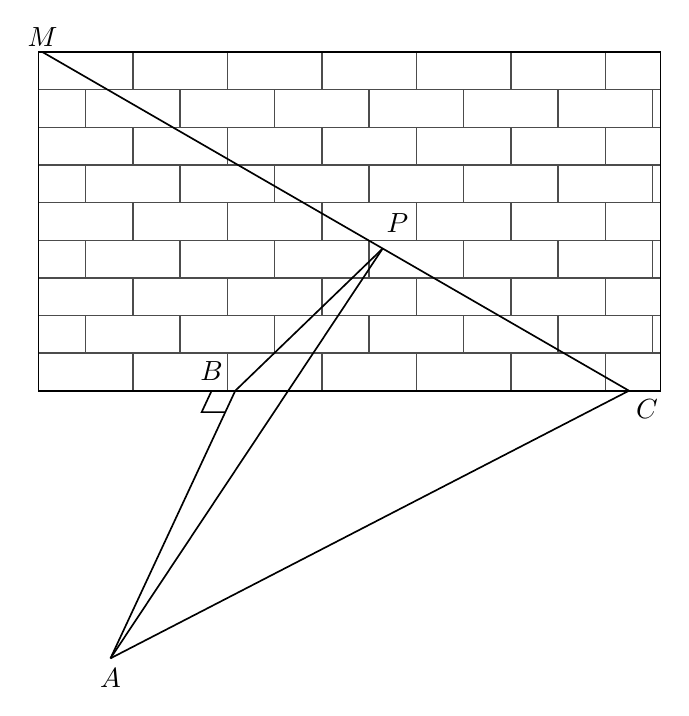
\begin{tikzpicture}[x=1cm,y=1cm,font=\normalsize,line width=.6pt,>=Latex]
  % wall plane: five courses of brick, staggered joints
  \coordinate (Wbl) at (-2.5,0);
  \coordinate (Wbr) at (5.4,0);
  \coordinate (Wtr) at (5.4,4.3);
  \coordinate (Wtl) at (-2.5,4.3);
  \draw[line width=.5pt,draw=black!70] (-2.5,0.477778)--(5.4,0.477778);
  \draw[line width=.5pt,draw=black!70] (-2.5,0.955556)--(5.4,0.955556);
  \draw[line width=.5pt,draw=black!70] (-2.5,1.433333)--(5.4,1.433333);
  \draw[line width=.5pt,draw=black!70] (-2.5,1.911111)--(5.4,1.911111);
  \draw[line width=.5pt,draw=black!70] (-2.5,2.388889)--(5.4,2.388889);
  \draw[line width=.5pt,draw=black!70] (-2.5,2.866667)--(5.4,2.866667);
  \draw[line width=.5pt,draw=black!70] (-2.5,3.344444)--(5.4,3.344444);
  \draw[line width=.5pt,draw=black!70] (-2.5,3.822222)--(5.4,3.822222);
  \draw[line width=.5pt,draw=black!70] (-1.300000,0.000000)--(-1.300000,0.477778);
  \draw[line width=.5pt,draw=black!70] (-0.100000,0.000000)--(-0.100000,0.477778);
  \draw[line width=.5pt,draw=black!70] (1.100000,0.000000)--(1.100000,0.477778);
  \draw[line width=.5pt,draw=black!70] (2.300000,0.000000)--(2.300000,0.477778);
  \draw[line width=.5pt,draw=black!70] (3.500000,0.000000)--(3.500000,0.477778);
  \draw[line width=.5pt,draw=black!70] (4.700000,0.000000)--(4.700000,0.477778);
  \draw[line width=.5pt,draw=black!70] (-1.900000,0.477778)--(-1.900000,0.955556);
  \draw[line width=.5pt,draw=black!70] (-0.700000,0.477778)--(-0.700000,0.955556);
  \draw[line width=.5pt,draw=black!70] (0.500000,0.477778)--(0.500000,0.955556);
  \draw[line width=.5pt,draw=black!70] (1.700000,0.477778)--(1.700000,0.955556);
  \draw[line width=.5pt,draw=black!70] (2.900000,0.477778)--(2.900000,0.955556);
  \draw[line width=.5pt,draw=black!70] (4.100000,0.477778)--(4.100000,0.955556);
  \draw[line width=.5pt,draw=black!70] (5.300000,0.477778)--(5.300000,0.955556);
  \draw[line width=.5pt,draw=black!70] (-1.300000,0.955556)--(-1.300000,1.433333);
  \draw[line width=.5pt,draw=black!70] (-0.100000,0.955556)--(-0.100000,1.433333);
  \draw[line width=.5pt,draw=black!70] (1.100000,0.955556)--(1.100000,1.433333);
  \draw[line width=.5pt,draw=black!70] (2.300000,0.955556)--(2.300000,1.433333);
  \draw[line width=.5pt,draw=black!70] (3.500000,0.955556)--(3.500000,1.433333);
  \draw[line width=.5pt,draw=black!70] (4.700000,0.955556)--(4.700000,1.433333);
  \draw[line width=.5pt,draw=black!70] (-1.900000,1.433333)--(-1.900000,1.911111);
  \draw[line width=.5pt,draw=black!70] (-0.700000,1.433333)--(-0.700000,1.911111);
  \draw[line width=.5pt,draw=black!70] (0.500000,1.433333)--(0.500000,1.911111);
  \draw[line width=.5pt,draw=black!70] (1.700000,1.433333)--(1.700000,1.911111);
  \draw[line width=.5pt,draw=black!70] (2.900000,1.433333)--(2.900000,1.911111);
  \draw[line width=.5pt,draw=black!70] (4.100000,1.433333)--(4.100000,1.911111);
  \draw[line width=.5pt,draw=black!70] (5.300000,1.433333)--(5.300000,1.911111);
  \draw[line width=.5pt,draw=black!70] (-1.300000,1.911111)--(-1.300000,2.388889);
  \draw[line width=.5pt,draw=black!70] (-0.100000,1.911111)--(-0.100000,2.388889);
  \draw[line width=.5pt,draw=black!70] (1.100000,1.911111)--(1.100000,2.388889);
  \draw[line width=.5pt,draw=black!70] (2.300000,1.911111)--(2.300000,2.388889);
  \draw[line width=.5pt,draw=black!70] (3.500000,1.911111)--(3.500000,2.388889);
  \draw[line width=.5pt,draw=black!70] (4.700000,1.911111)--(4.700000,2.388889);
  \draw[line width=.5pt,draw=black!70] (-1.900000,2.388889)--(-1.900000,2.866667);
  \draw[line width=.5pt,draw=black!70] (-0.700000,2.388889)--(-0.700000,2.866667);
  \draw[line width=.5pt,draw=black!70] (0.500000,2.388889)--(0.500000,2.866667);
  \draw[line width=.5pt,draw=black!70] (1.700000,2.388889)--(1.700000,2.866667);
  \draw[line width=.5pt,draw=black!70] (2.900000,2.388889)--(2.900000,2.866667);
  \draw[line width=.5pt,draw=black!70] (4.100000,2.388889)--(4.100000,2.866667);
  \draw[line width=.5pt,draw=black!70] (5.300000,2.388889)--(5.300000,2.866667);
  \draw[line width=.5pt,draw=black!70] (-1.300000,2.866667)--(-1.300000,3.344444);
  \draw[line width=.5pt,draw=black!70] (-0.100000,2.866667)--(-0.100000,3.344444);
  \draw[line width=.5pt,draw=black!70] (1.100000,2.866667)--(1.100000,3.344444);
  \draw[line width=.5pt,draw=black!70] (2.300000,2.866667)--(2.300000,3.344444);
  \draw[line width=.5pt,draw=black!70] (3.500000,2.866667)--(3.500000,3.344444);
  \draw[line width=.5pt,draw=black!70] (4.700000,2.866667)--(4.700000,3.344444);
  \draw[line width=.5pt,draw=black!70] (-1.900000,3.344444)--(-1.900000,3.822222);
  \draw[line width=.5pt,draw=black!70] (-0.700000,3.344444)--(-0.700000,3.822222);
  \draw[line width=.5pt,draw=black!70] (0.500000,3.344444)--(0.500000,3.822222);
  \draw[line width=.5pt,draw=black!70] (1.700000,3.344444)--(1.700000,3.822222);
  \draw[line width=.5pt,draw=black!70] (2.900000,3.344444)--(2.900000,3.822222);
  \draw[line width=.5pt,draw=black!70] (4.100000,3.344444)--(4.100000,3.822222);
  \draw[line width=.5pt,draw=black!70] (5.300000,3.344444)--(5.300000,3.822222);
  \draw[line width=.5pt,draw=black!70] (-1.300000,3.822222)--(-1.300000,4.300000);
  \draw[line width=.5pt,draw=black!70] (-0.100000,3.822222)--(-0.100000,4.300000);
  \draw[line width=.5pt,draw=black!70] (1.100000,3.822222)--(1.100000,4.300000);
  \draw[line width=.5pt,draw=black!70] (2.300000,3.822222)--(2.300000,4.300000);
  \draw[line width=.5pt,draw=black!70] (3.500000,3.822222)--(3.500000,4.300000);
  \draw[line width=.5pt,draw=black!70] (4.700000,3.822222)--(4.700000,4.300000);
  \draw (Wbl)--(Wbr)--(Wtr)--(Wtl)--cycle;

  % measured points: BC=20, AB=15, AC=25 (scale 0.25 cm per metre),
  % AB drawn in the oblique ground direction; angle BCM=30 degrees exactly.
  \coordinate (B) at (0,0);
  \coordinate (C) at (5,0);
  \coordinate (A) at (-1.585,-3.399);
  \coordinate (M) at (-2.447,4.3);
  \coordinate (P) at (1.872,1.806);
  \draw (B)--(A);
  \draw (B)--(P);
  \draw (A)--(P);
  \draw (A)--(C);
  \draw (C)--(M);

  % right angle between AB and the wall base at B
  \draw (-0.3,0)--(-0.427,-0.272)--(-0.127,-0.272);

  \node[anchor=south east,inner sep=0pt] at (-0.15,0.12) {$B$};
  \node[anchor=north west,inner sep=0pt] at (5.08,-0.10) {$C$};
  \node[anchor=north,inner sep=0pt] at (-1.585,-3.52) {$A$};
  \node[anchor=south,inner sep=0pt] at (-2.447,4.36) {$M$};
  \node[anchor=south west,inner sep=0pt] at (1.91,2.00) {$P$};
\end{tikzpicture}
